\section{Results}
\label{sec:results}

\subsection{Group A: Detection Sensitivity}

\begin{figure}[t]
\centering
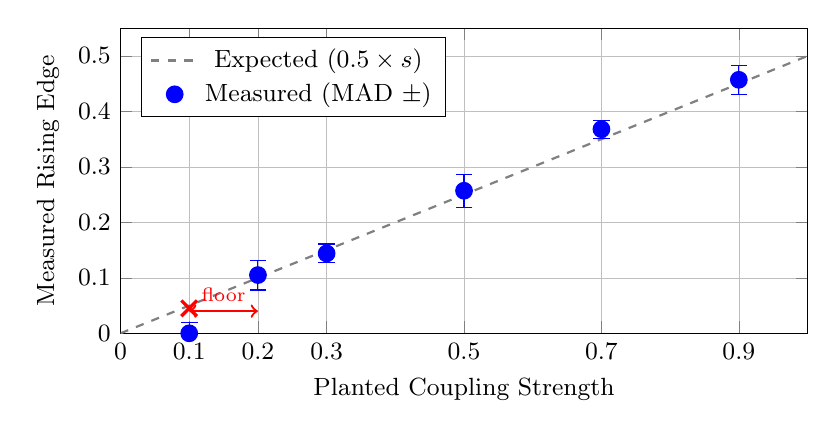
\begin{tikzpicture}
\begin{axis}[
  width=0.85\textwidth,
  height=0.45\textwidth,
  xlabel={Planted Coupling Strength},
  ylabel={Measured Rising Edge},
  xmin=0, xmax=1.0,
  ymin=0, ymax=0.55,
  xtick={0,0.1,0.2,0.3,0.5,0.7,0.9},
  xticklabels={0,0.1,0.2,0.3,0.5,0.7,0.9},
  ytick={0,0.1,0.2,0.3,0.4,0.5},
  grid=both,
  grid style={line width=.1pt, draw=gray!30},
  major grid style={line width=.2pt,draw=gray!50},
  legend pos=north west,
  legend style={font=\small},
  tick label style={font=\small},
  label style={font=\small},
]

% Expected line: y = 0.5 * x
\addplot[domain=0:1, dashed, gray, thick] {0.5*x};
\addlegendentry{Expected ($0.5 \times s$)}

% Measured points
\addplot[only marks, mark=*, mark size=3pt, color=blue,
  error bars/.cd, y dir=both, y explicit]
coordinates {
  (0.1, 0) +- (0,0.019)
  (0.2, 0.105) +- (0,0.027)
  (0.3, 0.144) +- (0,0.017)
  (0.5, 0.257) +- (0,0.030)
  (0.7, 0.368) +- (0,0.016)
  (0.9, 0.457) +- (0,0.026)
};
\addlegendentry{Measured (MAD $\pm$)}

% Detection floor annotation
\draw[<->, red, thick] (axis cs:0.1,0.04) -- (axis cs:0.2,0.04);
\node[red, font=\scriptsize, above] at (axis cs:0.15,0.04) {floor};

% Not detected marker
\addplot[only marks, mark=x, mark size=4pt, color=red, very thick]
coordinates {(0.1, 0.045)};

\end{axis}
\end{tikzpicture}
\caption{Detection sensitivity at noise $\sigma = 0.02$ (linear
coupling). Blue circles: measured rising edge with MAD error bars.
Dashed line: expected edge ($s \times 0.5$). Red $\times$: not
detected (below CFAR threshold). Measurement error consistently
below 5\%. Detection floor lies between coupling 0.1 and 0.2.}
\label{fig:sensitivity}
\end{figure}


\begin{table}[h]
\centering
\caption{Linear coupling strength sweep at noise $\sigma = 0.02$.}
\label{tab:strength}
\begin{tabular}{cccccc}
  \toprule
  Strength & Detected & Rising Edge & Expected & Error & MAD \\
  \midrule
  0.1 & \textbf{no}  & 0.045  & 0.05 & ---  & 0.019 \\
  0.2 & yes          & 0.105  & 0.10 & +5.2\% & 0.027 \\
  0.3 & yes          & 0.144  & 0.15 & $-$4.2\% & 0.017 \\
  0.5 & yes          & 0.257  & 0.25 & +2.9\% & 0.030 \\
  0.7 & yes          & 0.368  & 0.35 & +5.2\% & 0.016 \\
  0.9 & yes          & 0.457  & 0.45 & +1.4\% & 0.026 \\
  \bottomrule
\end{tabular}
\end{table}

The detection floor lies between coupling $0.1$ and $0.2$. At $0.1$,
the planted step amplitude ($0.05$) is comparable to the CFAR
threshold ($k \times \mathrm{MAD} \approx 3.0 \times 0.019 \approx
0.057$). The signal is present but below the noise-adaptive
threshold. Above $0.2$, detection is reliable with measurement error
consistently below $5\%$.

\subsection{Group B: Noise Robustness}

\begin{table}[h]
\centering
\caption{Noise robustness at coupling $s = 0.5$ (expected edge $0.25$).}
\label{tab:noise}
\begin{tabular}{cccccl}
  \toprule
  Noise $\sigma$ & Block & Detected & Edge & MAD & Note \\
  \midrule
  0.01  & 15 & yes & 0.237 & 0.034 & \\
  0.02  & 15 & yes & 0.257 & 0.030 & (Group A cell) \\
  0.05  & 15 & yes & 0.259 & 0.061 & \\
  0.10  & 15 & no  & ---   & 0.124 & signal $<$ threshold \\
  0.10  & 30 & no  & ---   & 0.093 & budget contrast: MAD drops, \\
        &    &     &       &      & still below threshold \\
  0.20  & 15 & no  & ---   & 0.253 & noise equals signal \\
  \bottomrule
\end{tabular}
\end{table}

Detection fails between noise $0.05$ and $0.10$. At noise $0.10$,
the asymptotic CFAR threshold ($k \to 3.0$ as $N \to \infty$) is
$0.30$, permanently above the signal ($0.25$). Doubling the block
size from 15 to 30 reduces MAD by $25\%$ and narrows the gap from
$63\%$ to $14\%$, but does not cross the threshold---the boundary
is governed by the SNR, not the observation budget alone.

\subsection{Group C: False Positives}

\begin{table}[h]
\centering
\caption{False positive test: coupling $s = 0.0$ (no edge exists).}
\label{tab:fpr}
\begin{tabular}{cccc}
  \toprule
  Noise $\sigma$ & Detected & MAD & Trials \\
  \midrule
  0.02  & no & 0.017 & 2 rounds \\
  0.10  & no & 0.116 & 1 round \\
  0.20  & no & 0.136 & 6 rounds \\
  \bottomrule
\end{tabular}
\end{table}

Zero false positives across the full noise range, including extreme
noise ($\sigma = 0.20$) where the MAD is an order of magnitude larger
than at the standard operating point. The threshold is conservative.

\subsection{Group D: Nonlinear Coupling Shapes}

\begin{table}[h]
\centering
\caption{Nonlinear shape generality at noise $\sigma = 0.02$.}
\label{tab:nonlinear}
\begin{tabular}{llcccc}
  \toprule
  Shape & Strength & Detected & Edge & MAD & Note \\
  \midrule
  Saturation  & 0.7 & yes & $-$0.113 & 0.028 & inverted step \\
  Threshold   & 0.7 & yes & \phantom{$-$}0.703 & 0.026 & discontinuous jump \\
  Polynomial  & 0.7 & yes & \phantom{$-$}0.517 & 0.028 & quadratic step \\
  \midrule
  Saturation  & 0.3 & \textbf{no}  & --- & 0.023 & step compressed below floor \\
  Threshold   & 0.3 & yes & \phantom{$-$}0.311 & 0.017 & large step from discontinuity \\
  Polynomial  & 0.3 & \textbf{no}  & --- & 0.005 & step below floor \\
  \bottomrule
\end{tabular}
\end{table}

All three nonlinear shapes are detected at coupling $0.7$.
Saturation produces an inverted step (the response at extreme
parameters is \emph{lower} than at mid-range); the detector
correctly identifies this via the absolute rising-edge test.

At coupling $0.3$, shape matters: threshold coupling is detected
(large step from the discontinuity), but saturation and polynomial
coupling fall below the detection floor. This is expected---nonlinear
shapes compress or redirect the step amplitude, and at low coupling
the compressed signal is indistinguishable from noise.
